\documentclass[11pt,a4paper]{article}

% ---------------------------------------------------------------------------
% Finite-batch selection between inherited chemical states under a shared
% limiting resource.
%
% Author metadata: set the three macros below before submission.
% They are deliberately left blank in this version.
% ---------------------------------------------------------------------------
\newcommand{\PaperAuthor}{}
\newcommand{\PaperAffiliation}{}
\newcommand{\PaperDate}{14 September 2026}

\usepackage[T1]{fontenc}
\usepackage[utf8]{inputenc}
\usepackage{lmodern}
\usepackage{microtype}
\usepackage[a4paper,margin=1.05in]{geometry}
\usepackage{amsmath,amssymb,amsthm,mathtools}
\usepackage{booktabs}
\usepackage{array}
\usepackage{enumitem}
\usepackage{xcolor}
\usepackage{graphicx}
\usepackage[obeyspaces,spaces]{url}
\usepackage[numbers,sort&compress]{natbib}
\usepackage[colorlinks=true,linkcolor=blue!55!black,citecolor=blue!55!black,urlcolor=blue!55!black]{hyperref}
\hypersetup{pdftitle={Finite-batch selection between inherited chemical states under a shared limiting resource},
  pdfkeywords={chemical heredity, compartment selection, resource competition, stochastic reaction networks, Foster--Lyapunov, protocells, Lean}}

\DeclareUrlCommand\lean{\urlstyle{tt}}
\setlist{itemsep=2pt,topsep=3pt}
\setlength{\emergencystretch}{1.5em}
\graphicspath{{figures/}}

\theoremstyle{plain}
\newtheorem{theorem}{Theorem}[section]
\newtheorem{proposition}[theorem]{Proposition}
\newtheorem{lemma}[theorem]{Lemma}
\newtheorem{corollary}[theorem]{Corollary}
\theoremstyle{definition}
\newtheorem{definition}[theorem]{Definition}
\newtheorem{assumption}[theorem]{Assumption}
\theoremstyle{remark}
\newtheorem{remark}[theorem]{Remark}

\newcommand{\R}{\mathbb R}
\newcommand{\N}{\mathbb N}
\newcommand{\E}{\mathbb E}
\newcommand{\Prb}{\mathbb P}
\newcommand{\cL}{\mathcal L}
\newcommand{\cS}{\mathcal S}
\newcommand{\cV}{\mathcal V}
\newcommand{\eps}{\varepsilon}
\newcommand{\chem}{\mathcal E_{\mathrm{chem}}}
\newcommand{\Esel}{\mathcal E_{\mathrm{sel}}}
\newcommand{\Etime}{\mathcal E_{\mathrm{time}}}
\newcommand{\tot}{\mathcal E_{\mathrm{tot}}}
\newcommand{\ind}{\mathbf 1}
\newcommand{\dd}{\mathrm d}
\newcommand{\Hs}{\mathrm H}
\DeclareMathOperator{\Bin}{Bin}

\title{Finite-batch selection between inherited chemical states\\under a shared limiting resource}
\author{\PaperAuthor\\[2pt]\small\PaperAffiliation}
\date{\PaperDate}

\begin{document}
\maketitle

\begin{abstract}
A chemical difference between compartments can change how fast they grow without changing how many compartments of each kind there are: in an asynchronously dividing population, accumulated size and offspring number are out of phase. We prove a quantitative finite-batch enrichment theorem for an explicit four-species count reaction network in which every compartment grows by drawing on one shared finite precursor pool while its resident feeds and removal channels remain maintained. Starting from any $h$ high-state and $\ell$ low-state newborns in explicit, nonempty, chemically certified regions around two stationary compositions, the high-state cell-count odds at the nutrient hitting time exceed $e^{s}h/\ell$ by the deadline $T$, except on an event of probability at most $\chem(N,M,T)+\Esel(N,s)+\Etime(N,\gamma,T)$, with all three terms explicit. At $s=0.1$ and $T=8/\gamma$ the error is at most $M(32+4/(21\gamma))e^{-cN}+e^{-19N/500000}+e^{-N/2500}$ with $c=1/(1.024\times10^{21})$, and a sharper retained bound is $O_{M,\gamma}(Ne^{-3cN})$. No fitness parameter is imposed: the growth advantage is the certified difference in resident concentration of the growth species, and chemical fidelity of every descendant is proved rather than assumed. The proof combines a size-position exponential that controls chemical recovery across divisions without any recovery clock, ancestral size totals that survive complementary division unchanged, and a single finite stopped law under which all failure branches are bounded without independence assumptions. For two founders the success event forces a high-state frequency of at least $4/7$. The finite stopped-law theorem and its quantitative consequences are verified in Lean~4; the identification with an ongoing nonexplosive count process up to the stopping event is a conventional localization argument. The copy numbers for which the bound is informative are astronomically large, and the result is a theorem about a specified effective model, not an experimental calibration.
\end{abstract}

\section{Introduction}\label{sec:intro}

Selection between compartments requires that a heritable difference change reproductive output. In compartmentalized chemistry the difference is a composition, reproduction is growth followed by division, and the output that matters is the number of compartments in each state. Whether a compositional difference translates into a difference in compartment number is not settled by comparing two growth rates. Three things intervene. Growth draws on resources that are shared, so the compartments are coupled and no compartment has an autonomous growth law. Division is asynchronous, so at any observation time the population is a mixture of division phases and a faster-growing lineage may hold more material but no more cells \citep{powell1956,taheri2015}. And the composition that confers the advantage must persist in every descendant through growth, dilution and random partition, which for finite molecule numbers is a probabilistic question in its own right \citep{segre2000,vasas2010,virgo2015}.

This paper answers the question for one explicit stochastic model and quantifies the answer. The model is a four-species count reaction network with thirteen resident channels, taken unchanged from an earlier chemical-copying study, in which a growth-linked species $z$ is consumed to build compartment size. Two stationary compositions of the resident chemistry differ in their $z$ concentration by a factor of about three. A batch consists of $M=h+\ell$ newborn compartments, $h$ of them in the high-$z$ state and $\ell$ in the low-$z$ state, sharing one finite pool of growth precursor. Every compartment grows at a rate proportional to its own $z$ count and to the remaining precursor concentration, divides into two complementary halves when its size doubles, and the batch ends when the pool is depleted to a fixed fraction. The main theorem states that, with explicit probability tending to one as the newborn copy number $N$ grows, the batch ends by a stated deadline, every compartment alive at that moment is still in the chemical state of its founder, and the ratio of high-state to low-state compartments has increased by a factor $e^{s}$ over its initial value. The three error terms, for chemistry, selection and deadline, are explicit functions of $N$, $M$, $\gamma$, $s$ and $T$.

\paragraph{Relation to prior work.}
That compartment growth can be driven by internal chemistry and that such growth can be competitive is established experimentally. Vesicles with higher internal osmotic load grow at the expense of neighbours \citep{chen2004}, encapsulated catalysts drive vesicle competition \citep{adamala2013}, and formose-driven droplets grow, compete for formaldehyde and transmit part of their growth-rate variation through division \citep{lu2024}. Active droplets with internal reactions grow and divide in a physical model of protocell proliferation \citep{zwicker2017}. On the theoretical side, compositional heredity in assemblies and autocatalytic networks has been analysed since \citet{segre2000} and \citet{szathmary1987}, with sharp criticism of its evolvability \citep{vasas2010,vasas2012}; \citet{nowak2008} study selection in prelife dynamics without templated replication; and \citet{matsubara2026} give conditions for Darwinian evolution in compartmentalized autocatalytic networks, including a Moran-type population with division at doubled volume and random removal, and shared-substrate competition inside their models. Experimental RNA networks show trade-offs between reproduction, variation and compositional persistence \citep{ameta2021}. Reviews of autocatalytic network theory \citep{kauffman1986,hordijk2004,blokhuis2020,nghe2015,serra2017} frame the general programme.

None of these works proves a finite-count probability theorem of the type given here, in which the chemical state of each descendant is controlled under the actual joint law of a resource-coupled, asynchronously dividing population and the outcome is a bound on cell-count odds. That is the contribution. We make no priority claim on the phenomenon of chemical selection, on asynchronous threshold division, or on shared-resource competition, all of which appear in the works cited. The literal reaction rates and size thresholds of the model are not calibrated to any experiment.

\paragraph{Method.}
All probabilities are computed under one finite continuous-time Markov jump law \citep{kurtz1972,gillespie1977,andersonkurtz2015} that is stopped at the first chemical flag or at the nutrient endpoint and retains an absorbing record of the terminal event. Failure probabilities are bounded by Foster--Lyapunov-type comparison functions \citep{meyntweedie1993,gupta2014,kuntz2019} evaluated on that finite law; the comparison functions are exponentials of certified quadratic energies, of a size-position coordinate, and of logarithms of ancestral size totals. Three ingredients are, to our knowledge, new in this setting. First, a position exponential $e^{\lambda(m-2N)}e^{\alpha NE}$ in the compartment size $m$ makes the chemical energy $E$ of a compartment decrease on average all the way to division, so that two admitted daughters cost no more than their parent and no recovery clock or birth reserve is needed. Second, the total size of all descendants of one founder is conserved by complementary division and grows at a rate that is, on chemically safe states, sandwiched between explicit multiples of itself; a normalized exponential of a logarithmic combination of these ancestral totals is a supermartingale, and its endpoint value converts size odds into cell-count odds at the explicit cost of a factor two for division phase. Third, all exceptional events are handled by a union bound under the same law, so that no independence between compartments, between daughters, or between failure types is assumed anywhere. Every quantitative inequality is symbolic in $N$, $M$, $\gamma$, $s$ and $T$; no state enumeration, sampled trajectory or floating-point evaluation enters the proof.

\paragraph{Verification.}
The finite stopped-law theorem, its instantiation at the two source compositions, and the quantitative consequences of Section~\ref{sec:results} are checked in Lean~4 with Mathlib \citep{demoura2021,mathlib2020}. Appendix~\ref{app:formal} lists the declarations, the receipts and the precise boundary between machine-checked and conventional statements. The conventional part is the nonexplosion and coupling argument of Section~\ref{sec:localization} that identifies the stopped law with an unrestricted count process up to the stopping event, and the interpretations of Section~\ref{sec:discussion}.

\paragraph{Organization.}
Section~\ref{sec:model} defines the model and the success event. Section~\ref{sec:results} states the theorems and their consequences. Sections~\ref{sec:finitelaw}--\ref{sec:assembly} prove them. Section~\ref{sec:localization} gives the ongoing-process interpretation. Section~\ref{sec:numbers} evaluates the bounds and Section~\ref{sec:discussion} discusses scope and open questions. Appendix~\ref{app:cert} records the source certificate, Appendix~\ref{app:ineq} the elementary inequalities, and Appendix~\ref{app:formal} the formal source map.

\section{The effective count model}\label{sec:model}

\subsection{Resident channels and compartment size}
A compartment carries resident counts $n=(n_A,n_B,n_z,n_\Hs)\in\N^4$ and an integer size $m\geq1$. Concentrations are $x=n/m$. The size $m$ is a coarse-grained coordinate in units for which the compartment volume is proportional to $m$; it is not derived from membrane area or membrane mass, and this proportionality is an assumption of the model. A newborn has size $N$. With $\eps=10^{-5}$ and $\eta=10^{-4}$, the thirteen resident channels of Table~\ref{tab:rates} specify every resident transition. All propensities are the literal count propensities, with falling-factorial factors for identical reactants and zero propensity when a reactant is absent.

\begin{table}[ht]
\centering
\caption{Resident count propensities at size $m$; $\eps=10^{-5}$, $\eta=10^{-4}$.}
\label{tab:rates}
\begin{tabular}{cll}
\toprule
Channel & Effective transition & Propensity\\
\midrule
1 & $A\to B+z$ & $n_A$\\
2 & $B+z\to A$ & $n_Bn_z/m$\\
3 & $z\to\Hs$ & $16n_z$\\
4 & $\Hs\to z$ & $n_\Hs$\\
5 & $\Hs\to2z$ & $n_\Hs$\\
6 & $2z\to\Hs$ & $2n_z(n_z-1)/m$\\
7 & $\varnothing\to A$ & $6m$\\
8 & $A\to\varnothing$ & $n_A$\\
9 & $\varnothing\to B$ & $27m$\\
10 & $B\to\varnothing$ & $n_B$\\
11 & $B\to2A$ & $\eps n_B$\\
12 & $2A\to B$ & $\eps n_A(n_A-1)/m$\\
13 & $\Hs\to\varnothing$ & $\eta n_\Hs$\\
\bottomrule
\end{tabular}
\end{table}

These are effective open-system channels. The pairs $z\rightleftarrows\Hs$ and $\Hs\rightleftarrows2z$ cannot both conserve positive resident masses without omitted species, and we claim no atom-balanced or thermodynamically autonomous realization. Maintained feeds (channels 7 and 9), removals (8, 10, 13) and any omitted driving reservoirs are part of the model's external conditions. The theorem is about this propensity table; adding reverse channels would change it.

\subsection{Shared growth precursor and complementary division}
Let $h,\ell\geq1$ be the founder numbers and $M=h+\ell$. The population starts with $M$ newborns of size $N$, a common precursor count $Q_0=4NM$ and an external volume parameter $\Omega=4NM$. Compartment $j$ grows by the event
\begin{equation}\label{eq:growth}
\text{rate }\gamma\frac{Q}{\Omega}n_{z,j},\qquad (Q,n_{z,j},m_j)\mapsto(Q-1,n_{z,j}-1,m_j+1),
\end{equation}
which is disabled when $Q=0$ or $n_{z,j}=0$. One molecule of $z$ and one unit of precursor are converted into one unit of size. The precursor is the only finite external quantity; the resident supplies and removals of Table~\ref{tab:rates} are maintained throughout. The parameter $\gamma$ has units of inverse time once the reference unit of $Q/\Omega$ is fixed; the theorem assumes $0<\gamma\leq10^{-11}$ in the time unit in which the resident propensities of Table~\ref{tab:rates} are expressed, that is, growth is slow compared with resident chemistry.

When a growth event brings the size to $2N$, the same event replaces the parent by two compartments of size $N$. Conditional on the post-growth resident count $n$, draw $d_i\sim\Bin(n_i,1/2)$ independently over the four species and give $d$ to one daughter and $n-d$ to the other. The two daughters are complementary, not independent. Both inherit the parent's ancestral tag. The allocation law is
\begin{equation}\label{eq:partition}
w_n(d)=\prod_{i=1}^{4}2^{-n_i}\binom{n_i}{d_i},\qquad0\leq d_i\leq n_i.
\end{equation}
Division is processed even when the triggering growth event is the one that reaches the nutrient endpoint $Q=NM$. Figure~\ref{fig:model} summarizes the model.

\begin{figure}[ht]
\centering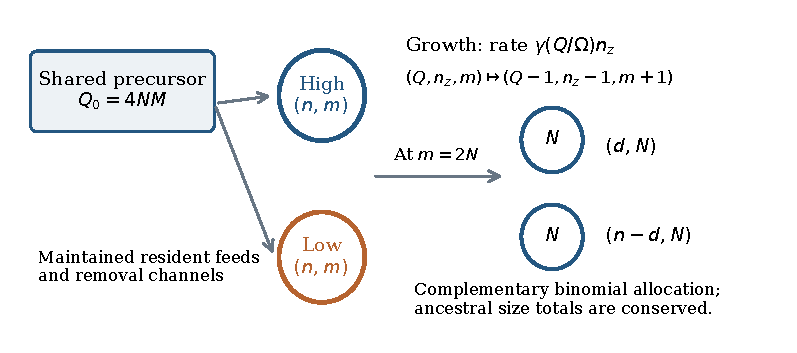
\includegraphics[width=.92\linewidth]{model.pdf}
\caption{The fixed-batch model. All compartments draw growth precursor from one pool; each grows at a rate set by its own resident $z$ count and the remaining precursor concentration. At size $2N$ the parent is replaced by two complementary newborns of size $N$ carrying its ancestral tag.}
\label{fig:model}
\end{figure}

\subsection{Stationary compositions, newborn regions and readout}\label{sec:source}
The concentration drift of the resident channels in the large-$m$ limit is
\begin{equation}\label{eq:drift}
f(x)=\begin{pmatrix}
6-2x_A+x_Bx_z+2\eps(x_B-x_A^2)\\
27+x_A-(1+x_z)x_B-\eps(x_B-x_A^2)\\
x_A-x_Bx_z-16x_z-4x_z^2+3x_\Hs\\
16x_z+2x_z^2-(2+\eta)x_\Hs
\end{pmatrix}.
\end{equation}
The proof uses the finite-count law with its $1/m$ corrections, not this limiting drift; the drift only locates the two compositions. For a scalar $z$ put
\begin{align*}
B(z)&=\frac{60}{z+2},& K(z)&=\frac{2(1+2\eta)z^2-16(1-\eta)z}{2+\eta},\\
A(z)&=zB(z)+K(z),& H(z)&=\frac{16z+2z^2}{2+\eta}.
\end{align*}
Along the curve $x(z)=(A(z),B(z),z,H(z))$ the third and fourth coordinates of $f$ vanish identically, the second equals the residual $r(z)=27-(1+\eps)B(z)+K(z)+\eps A(z)^2$, and the first equals $-2r(z)$. The residual changes sign on each of the intervals
\begin{equation}\label{eq:roots}
z_L\in[0.99579401232,\,0.99579401233],\qquad z_H\in[2.97636724376,\,2.97636724377],
\end{equation}
so by continuity there are stationary compositions $x_L^*=x(z_L)$ and $x_H^*=x(z_H)$ with $f(x_i^*)=0$. Only the exact rational endpoint signs and continuity are used; no numerical root is assumed. The two compositions differ mainly in $z$, by a factor of about three.

For each tag $i\in\{L,H\}$ let $E_i(x)=(x-x_i^*)^{\!\top}P_i(x-x_i^*)$ with the positive definite rational matrices $P_i$ of Appendix~\ref{app:cert}. Define
\begin{equation}\label{eq:constants}
\begin{gathered}
b=\frac1{32000000},\qquad a=\frac b{16}=\frac1{512000000},\qquad u=\alpha aN=2cN,\\
\alpha=10^{-12},\qquad \lambda=10^{-15},\qquad \delta=10^{-6},
\end{gathered}
\end{equation}
with $c=1/(1.024\times10^{21})$. A \emph{newborn of tag $i$} is a compartment with $m=N$ and $E_i(n/N)\leq4a$. Heterogeneous founders inside these closed regions are allowed. For $N\geq10^{12}$ each region contains an integer count (Appendix~\ref{app:cert}), so the hypotheses of the theorem are never vacuous.

Ancestral tags are bookkeeping. The measured chemical state is the sign of the readout $10n_z-n_B$: positive means high, negative means low. Whenever $E_i<b$ the readout has the sign of tag $i$, and
\begin{equation}\label{eq:zsafe}
0.99\leq x_z\leq1.01\quad(i=L),\qquad 2.97\leq x_z\leq3\quad(i=H).
\end{equation}
A chemically successful history therefore turns ancestry counts into counts of measured chemical states.

\subsection{The stopped event}\label{sec:stopped}
After every reaction, inspect the updated compartment. Stop with an \emph{outer failure} if its energy is at least $b$. At a division, stop with a \emph{division-energy failure} if the post-growth parent energy exceeds $2a$, and with a \emph{partition failure} if either daughter has energy at least $4a$. Otherwise, stop with \emph{nutrient success} when the growth event brings $Q$ to $NM$. Chemical flags take priority over nutrient success on a simultaneous event. Let $\tau$ be the nutrient hitting time and $\sigma$ the first chemical flag.

Write $C_H(t)$ and $C_L(t)$ for the number of live compartments of each tag. For a real gain $s$ and a horizon $T\geq0$, the \emph{successful enrichment event} $\cS_{s,T}$ is: $\tau\leq T$, no chemical flag up to and including the endpoint transition, every live compartment at $\tau$ has the readout of its tag, both tags are present at $\tau$, and
\begin{equation}\label{eq:gain}
\frac{C_H(\tau)}{C_L(\tau)}\geq e^{s}\frac{h}{\ell}.
\end{equation}
The finite law retains an absorbing record of the terminal event, including the physical outcome state of the endpoint transition, so evaluating it at time $T$ records success \emph{by} $T$. The theorem asserts nothing about the population after $\tau$; Section~\ref{sec:localization} makes the ongoing-process reading precise.

\section{Main results}\label{sec:results}

Define the raw chemical error
\begin{equation}\label{eq:raw}
\chem(N,M,T)=7Me^{-12u}+\frac{MT}{84}ue^{-31u/2}+Me^{2u-\lambda N}+\frac{MT}{84}ue^{-3u/2}+24Me^{-N\delta^2/35},
\end{equation}
and, with $\theta=1/1000$, the selection and deadline tails
\begin{equation}\label{eq:tails}
\Esel(N,s)=\exp\{-\theta N[\tfrac35\log4-\log2-s]\},\qquad \Etime(N,\gamma,T)=\exp\{-\theta N[\tfrac{9}{40}\gamma T-\log4]\}.
\end{equation}

\begin{theorem}[Finite-batch selection, general gain and deadline]\label{thm:family}
There are stationary compositions $x_L^*,x_H^*$ with $z_L,z_H$ in the intervals \eqref{eq:roots}. Fix integers $h,\ell\geq1$, $M=h+\ell$, a growth coupling $0<\gamma\leq10^{-11}$ and an integer $N\geq1.4\times10^{20}$. Both newborn regions are nonempty. Start the population law of Section~\ref{sec:model} from any $h$ newborns of tag $H$ and $\ell$ newborns of tag $L$ with $Q_0=\Omega=4NM$. Then for every real $s$ and every $T\geq0$,
\begin{equation}\label{eq:main}
\Prb(\cS_{s,T})\geq1-\chem(N,M,T)-\Esel(N,s)-\Etime(N,\gamma,T).
\end{equation}
\end{theorem}

The inequality \eqref{eq:main} holds for all $s$ and $T$; it is informative only when the two population margins $\frac35\log4-\log2-s=\frac15\log2-s$ and $\frac9{40}\gamma T-\log4$ are positive and the total error is below one.

\begin{theorem}[Fixed gain at the natural deadline]\label{thm:main}
Under the hypotheses of Theorem~\ref{thm:family}, at $s=0.1$ and $T=8/\gamma$,
\begin{equation}\label{eq:original}
\Prb(\cS_{0.1,8/\gamma})\geq1-M\Big(32+\frac{4}{21\gamma}\Big)e^{-cN}-e^{-19N/500000}-e^{-N/2500},
\end{equation}
and for fixed $M$ and $\gamma$ the right-hand side tends to one as $N\to\infty$.
\end{theorem}

\begin{corollary}[Frequency; two founders]\label{cor:frequency}
Let $p_0=h/M$ and $p_\tau=C_H(\tau)/(C_H(\tau)+C_L(\tau))$. On $\cS_{s,T}$,
\begin{equation}\label{eq:frequency}
p_\tau\geq\frac{e^{s}p_0}{1-p_0+e^{s}p_0},\qquad p_\tau-p_0\geq\frac{p_0(1-p_0)(e^{s}-1)}{1+p_0(e^{s}-1)}.
\end{equation}
If $h=\ell=1$ and $s=0.1$, then $p_\tau\geq4/7$ on $\cS_{0.1,T}$.
\end{corollary}

\begin{corollary}[Sharper chemical certificates]\label{cor:sharp}
For all $M,T\geq0$ and $N\in\N$,
\begin{equation}\label{eq:sharp}
\chem(N,M,T)\leq M\Big(32+\frac{Tu}{42}\Big)e^{-3u/2},\qquad \chem(N,M,T)\leq M\Big(32+\frac T{21}\Big)e^{-u}.
\end{equation}
In particular $\chem(N,M,8/\gamma)=O_{M,\gamma}(Ne^{-3cN})$, and the second bound is a pure exponential with exponent $2c$. These are upper bounds on the certified error; no matching lower bound on the true failure probability is claimed.
\end{corollary}

\begin{proposition}[Sufficient copy numbers and joint scaling]\label{prop:thresholds}
\begin{enumerate}[label=(\roman*)]
\item For $\eps_0>0$, the total error in \eqref{eq:original} is at most $\eps_0$ whenever $N$ is at least the maximum of
\begin{equation}\label{eq:threshold}
1.4\times10^{20},\qquad \frac1c\log\frac{3M(32+4/(21\gamma))}{\eps_0},\qquad \frac{500000}{19}\log\frac3{\eps_0},\qquad 2500\log\frac3{\eps_0}.
\end{equation}
With the pure-exponential certificate of Corollary~\ref{cor:sharp} the second entry may be replaced by $(2c)^{-1}\log[3M(32+8/(21\gamma))/\eps_0]$.
\item Let $M_N\geq2$ and $0<\gamma_N\leq10^{-11}$ vary with $N$. If
\begin{equation}\label{eq:scaling}
\log M_N+\log(1/\gamma_N)+\log(N+1)-3cN\longrightarrow-\infty,
\end{equation}
then $\chem(N,M_N,8/\gamma_N)\to0$, and the total error in \eqref{eq:original} with $(M,\gamma)=(M_N,\gamma_N)$ tends to zero.
\end{enumerate}
\end{proposition}

\begin{remark}
Theorem~\ref{thm:main} is the form in which the result was first proved; Theorem~\ref{thm:family} is obtained from the same proof by carrying $s$ and $T$ as parameters. The three error terms are of different natures. The chemical term counts the certified reliability budget consumed by $M$ compartments over a physical time $T$: it grows linearly in $M$ and $T$ and decays exponentially in $N$. The selection term is the price of demanding a logarithmic gain $s$ in cell-count odds when only $\frac15\log2\approx0.1386$ of logarithmic gain in size odds is certified after paying for division phase. The deadline term is the price of demanding the endpoint by $T$ when the population needs at least $\frac{40}{9}\log4/\gamma\approx6.16/\gamma$ of physical time on the certified growth rates. More time weakens the deadline term but strengthens the chemical term.
\end{remark}

\section{The finite stopped law}\label{sec:finitelaw}

\subsection{Conservation identities}
Let $W=\sum_jm_j$ be the total size of the live population, $D$ the number of divisions so far, and $C=C_H+C_L$ the number of live compartments.

\begin{lemma}[Conservation]\label{lem:conservation}
Resident reactions leave $Q$ and $W$ unchanged; a growth event decrements $Q$ and increments $W$ by one; a division leaves $W$ unchanged and increments $C$ and $D$ by one. Hence along every path up to and including the endpoint transition
\begin{equation}\label{eq:conservation}
Q+W=5NM,\qquad C=M+D,\qquad W(\tau)=4NM.
\end{equation}
Every live compartment, including both endpoint daughters, satisfies $N\leq m<2N$. Consequently $2M<C\leq4M$ at the endpoint, $C\leq4M$ and $D\leq3M$ always, and $C<4M$, $D<3M$ in every continuing state ($Q>NM$).
\end{lemma}
\begin{proof}
The three transition rules of Section~\ref{sec:model} give the increments directly; the identities follow by induction along the path with $Q_0=4NM$, $W_0=NM$, $C_0=M$, $D_0=0$. Growth from $m<2N$ either gives $m+1<2N$ or triggers division to two compartments of size $N$, so the size bounds are preserved. From $NC\leq W\leq2NC$ and $W\leq4NM$ we get $C\leq4M$; the strict versions use $W<4NM$ in a continuing state and $W=4NM$ with $m<2N$ at the endpoint.
\end{proof}

\subsection{The finite active domain and the stopped kernel}
Before any chemical flag every compartment satisfies $E_i<b$, and the quadratic lower bound $E_i\geq\|x-x_i^*\|^2/200$ together with the coordinates of $x_i^*$ (Appendix~\ref{app:cert}) forces $n_k\leq70N$ for each resident species. With Lemma~\ref{lem:conservation} this bounds the number of compartments, all counts, all sizes and $Q$, so the set $\mathcal D$ of \emph{active} population states is finite.

An \emph{event} from an active state selects one live compartment $j$ and either one of the thirteen resident channels or the growth channel together with a complementary draw $d$. Its rate is the corresponding propensity, times $w_n(d)$ in the growth-with-division case. The event is inspected as in Section~\ref{sec:stopped}. If no flag and no endpoint is raised, the process moves to the outcome state, which is again in $\mathcal D$ because positive-rate transitions preserve the bounds above and the energy test was passed. Otherwise the process moves to an absorbing \emph{terminal record} that stores the event and hence its physical outcome state. Let $\cL$ be the generator of this finite stopped chain on $\mathcal D\cup\{\text{terminal records}\}$; it vanishes on terminal records. Impossible transitions (missing reactants, $Q=0$) have rate zero and are never counted as success or as failure.

Choose a clock $q>0$ that dominates every total outgoing rate and satisfies $q\geq\frac9{40000}N\gamma$. The uniformized kernel $P=I+\cL/q$ is stochastic, and the physical-time law is the Poissonized kernel
\begin{equation}\label{eq:uniformize}
P_t=e^{-qt}\sum_{k\geq0}\frac{(qt)^k}{k!}P^k .
\end{equation}
All probabilities in Theorems~\ref{thm:family} and \ref{thm:main} are expectations of indicator functions under $P_T$ started at the founder state. This is the standard construction of a finite continuous-time chain from its jump rates \citep{norris1997}; its equality in law with the minimal jump process of Section~\ref{sec:model} up to the stopping time is discussed in Section~\ref{sec:localization}.

\subsection{Comparison lemmas}
The following two facts are the only probabilistic tools used. Both are proved by iterating the kernel inequality and summing the Poisson series; no independence enters.

\begin{lemma}[Drift and barrier]\label{lem:barrier}
Let $V\geq0$ be a function on the stopped state space with $\cL V\leq B$ pointwise for a constant $B\geq0$, and let $F$ be a set of terminal records on which $V\geq A>0$. Then for every $t\geq0$ and starting state $x_0$,
\begin{equation}\label{eq:driftbound}
A\,\Prb_{x_0}(X_t\in F)\leq V(x_0)+tB.
\end{equation}
If instead $\cL V\leq-\kappa V$ with $0\leq\kappa\leq q$, then $\E_{x_0}V(X_t)\leq e^{-\kappa t}V(x_0)$.
\end{lemma}
\begin{proof}
From $PV=V+\cL V/q\leq V+B/q$ and $P\geq0$, induction gives $P^kV\leq V+kB/q$, and \eqref{eq:uniformize} with $\sum_ke^{-qt}(qt)^kk/(k!q)=t$ gives $P_tV\leq V+tB$. Since $A\ind_F\leq V$ pointwise, $A\,P_t\ind_F\leq P_tV$. In the second case $PV\leq(1-\kappa/q)V$, hence $P^kV\leq(1-\kappa/q)^kV$, and the Poisson sum equals $e^{-\kappa t}$.
\end{proof}

\begin{lemma}[Union bound]\label{lem:union}
If the complement of the success set is covered by sets $F_1,\dots,F_k$, then $\Prb_{x_0}(\cS)\geq1-\sum_i\Prb_{x_0}(X_T\in F_i)$.
\end{lemma}

To apply Lemma~\ref{lem:barrier} to a terminal record, a comparison function is extended to records by assigning either a barrier value (for the failure type being bounded), the value at the physical outcome state, or zero. Because records are absorbing, $\cL$ vanishes there, so the drift bound need only be checked on active states, where it reads
\begin{equation}\label{eq:activedrift}
\cL V(x)=\sum_{\text{events }e}\text{rate}(e)\,[V(\text{next}(x,e))-V(x)].
\end{equation}
If $V(\text{next}(x,e))\leq\widetilde V(x,e)$ for a bound $\widetilde V$ that is easier to compute (typically the value at the raw outcome state before inspection), then $\cL V(x)\leq\sum_e\text{rate}(e)[\widetilde V(x,e)-V(x)]$. This is how the boundary behaviour of every observable below is handled.

\section{Chemical reliability}\label{sec:chemical}

Throughout this section $\beta=\gamma Q/\Omega$ denotes the current growth coefficient. In the active domain $0\leq\beta\leq\gamma\leq10^{-11}$, so every source inequality that is uniform in $\beta\in[0,10^{-11}]$ applies statewise, with no conditioning on the future resource path.

\subsection{The source-local estimate}
For a compartment of tag $i$ with $N\leq m<2N$ and $E_i<b$ put $Z=e^{\alpha NE_i}$ and $k=u/672$. Let $\cL_{\mathrm{cell}}$ be the single-compartment generator: the thirteen resident channels of Table~\ref{tab:rates} at size $m$ plus the growth channel \eqref{eq:growth} at coefficient $\beta$, acting on functions of $(n,m)$ before inspection. The source certificate of Appendix~\ref{app:cert} gives, for $N\geq1.4\times10^{20}$,
\begin{equation}\label{eq:local}
\cL_{\mathrm{cell}}Z\leq-kZ+2ke^{u/2},\qquad Z(\text{post-growth state})\leq2Z .
\end{equation}
The first inequality is the affine recovery estimate: away from the composition the energy decreases exponentially fast, and near it the drift is bounded by the constant $2ke^{u/2}$. The second says that one growth event, which dilutes all four concentrations by the factor $m/(m+1)$ and removes one $z$, changes the exponential by at most a factor two; it holds also for the growth event that triggers division. In the population generator, an event in compartment $j'\neq j$ does not change $(n_j,m_j)$, so a function of one compartment feels only that compartment's channels.

\subsection{A position exponential and division control}
\begin{lemma}[Position exponential]\label{lem:spatial}
Define $V(n,m)=e^{\lambda(m-2N)}Z(n,m)$ on compartments with $N\leq m<2N$ and $E_i<b$. Then
\begin{equation}\label{eq:spatialdrift}
\cL_{\mathrm{cell}}V\leq-\frac k2V+2ke^{u/2}.
\end{equation}
\end{lemma}
\begin{proof}
Resident channels do not change $m$, so on them $V$ behaves as $g Z$ with $g=e^{\lambda(m-2N)}$ frozen. The growth channel changes both factors, and the product rule for a single jump gives the exact identity
\[
\cL_{\mathrm{cell}}V=g\,\cL_{\mathrm{cell}}Z+\beta n_z\,g\,(e^{\lambda}-1)\,Z(\text{post-growth state}).
\]
Use $g\leq1$, $n_z\leq8N$ on the safe box, $e^\lambda-1\leq2\lambda$ and the growth ratio in \eqref{eq:local}: the second term is at most $32\beta\lambda N\,gZ$. Since $k/2=\alpha aN/1344$, the exact inequality $32\gamma\lambda\leq\alpha a/1344$ gives $32\beta\lambda N\leq k/2$, and adding the first part of \eqref{eq:local} multiplied by $g\leq1$ gives \eqref{eq:spatialdrift}.
\end{proof}

The point of the position factor is what happens at division. At a division-energy failure the raw post-growth parent has $m=2N$, so $g=1$, and $E_i>2a$, so $V=Z>e^{2u}$. At an admitted division the parent has $m=2N$, $g=1$ and $E_i\leq2a$, so $V\geq1$, while each admitted daughter has $m=N$ and $E_i<4a$, so $V<e^{4u-\lambda N}$. The constants \eqref{eq:constants} and $N\geq1.4\times10^{20}$ give $2e^{4u-\lambda N}\leq1$ (Appendix~\ref{app:cert}). Replacing an admitted parent by its two admitted daughters therefore never increases the sum of $V$ over the population. This is why no recovery clock at random birth times and no birth reserve are needed for the division-energy branch.

\begin{lemma}[Division-energy failures]\label{lem:division}
Let $F_D$ be the set of division-energy terminal records. Then
\begin{equation}\label{eq:divisionfail}
\Prb(F_D\text{ by }T)\leq Me^{2u-\lambda N}+\frac{MT}{84}ue^{-3u/2}.
\end{equation}
\end{lemma}
\begin{proof}
Let $V_{\mathrm{pop}}$ be the sum of $V$ over live compartments on active states, $e^{2u}$ on records in $F_D$, and zero on other records. On an active state every event's next value is at most the sum of $V$ over the raw outcome: this is an equality for resident and non-dividing growth events, the daughter comparison above for admitted divisions, the barrier inequality $e^{2u}<V(\text{raw parent})$ for records in $F_D$, and trivial for zero-valued records. Hence by \eqref{eq:activedrift} and Lemma~\ref{lem:spatial}, $\cL V_{\mathrm{pop}}\leq\sum_j2ke^{u/2}\leq8Mke^{u/2}$ using $C\leq4M$. Initially every founder has $m=N$ and $E_i\leq4a$, so $V_{\mathrm{pop}}(x_0)\leq Me^{4u-\lambda N}$. Lemma~\ref{lem:barrier} with $A=e^{2u}$ and $B=8Mke^{u/2}=\frac{Mu}{84}e^{u/2}$ gives \eqref{eq:divisionfail}.
\end{proof}

\subsection{Outer exits}
\begin{lemma}[Outer failures]\label{lem:outer}
Let $F_O$ be the set of outer terminal records. Then
\begin{equation}\label{eq:outerfail}
\Prb(F_O\text{ by }T)\leq7Me^{-12u}+\frac{MT}{84}ue^{-31u/2}.
\end{equation}
\end{lemma}
\begin{proof}
Use the observable $\sum_jZ_j+(6M-2D)e^{4u}$ on active states, $e^{\alpha Nb}=e^{16u}$ on records in $F_O$ and zero elsewhere. The reserve is nonnegative because $D\leq3M$. An admitted division removes the parent's $Z_j\geq1$ and adds two daughters with $Z<e^{4u}$ each, paid by the reserve decrement $2e^{4u}$. At an outer record the raw updated compartment has $E_i\geq b$, so its $Z$ alone is at least the barrier. Dropping the negative term in \eqref{eq:local}, the drift is at most $8Mke^{u/2}$ as before. The initial value is at most $Me^{4u}+6Me^{4u}=7Me^{4u}$. Lemma~\ref{lem:barrier} with $A=e^{16u}$ gives \eqref{eq:outerfail}.
\end{proof}

\subsection{Complementary partition}
\begin{lemma}[Partition failures]\label{lem:partition}
If the post-growth parent has $m=2N$ and $E_i\leq2a$, then
\begin{equation}\label{eq:partitionfail}
\sum_dw_n(d)\,\ind\{E_i(d/N)\geq4a\text{ or }E_i((n-d)/N)\geq4a\}\leq\eps_P:=8e^{-N\delta^2/35}.
\end{equation}
Consequently, with $F_P$ the set of partition terminal records,
\begin{equation}\label{eq:partitionglobal}
\Prb(F_P\text{ by }T)\leq3M\eps_P=24Me^{-N\delta^2/35}.
\end{equation}
\end{lemma}
\begin{proof}
Each daughter concentration coordinate is $d_i/N$ with $d_i\sim\Bin(n_i,1/2)$ and $n_i\leq70N$ on the safe box; its deviation from the parent concentration $n_i/(2N)$ exceeds $\delta$ with probability at most $2e^{-2N\delta^2/70}$ by the binomial moment generating function bound \citep{hoeffding1963}. A union over the four coordinates gives $\eps_P$ for the event that some coordinate deviates by more than $\delta$. Outside this event the daughter deviation vector $v$ has $\|v\|^2\leq4\delta^2$, so $E_i(v)\leq42\|v\|^2\leq168\delta^2<a/4$ by the margin $42\cdot16\delta^2<a$, and the Cauchy--Schwarz bound $E_i(y+v)\leq(\sqrt{E_i(y)}+\sqrt{E_i(v)})^2\leq(\sqrt{2a}+\sqrt{a}/2)^2<4a$ takes a parent energy at most $2a$ to daughter energies below $4a$. The second daughter's deviation vector is the negative of the first, so both daughters are covered by the same event; nothing is assumed about independence between the daughters. For \eqref{eq:partitionglobal}, use the observable $(3M-D)\eps_P$ on active states, $1$ on records in $F_P$ and zero elsewhere. On an event that triggers an admitted or failed division from a parent with $E_i\leq2a$, the expected next value is at most $\eps_P\cdot1+(1-\eps_P)(3M-D-1)\eps_P\leq(3M-D)\eps_P$ by \eqref{eq:partitionfail}; a parent with $E_i>2a$ produces a division-energy record of value zero; all other events leave the value unchanged. So the generator is nonpositive and Lemma~\ref{lem:barrier} with $A=1$, $B=0$ gives \eqref{eq:partitionglobal}, since $D\geq0$ initially.
\end{proof}

\begin{proposition}[Chemical error]\label{prop:chem}
$\Prb(F_O\cup F_D\cup F_P\text{ by }T)\leq\chem(N,M,T)$ with $\chem$ as in \eqref{eq:raw}.
\end{proposition}
\begin{proof}
Add \eqref{eq:outerfail}, \eqref{eq:divisionfail} and \eqref{eq:partitionglobal}; the three sets are disjoint records under the same law.
\end{proof}

\section{Selection and deadline}\label{sec:selection}

\subsection{Ancestral size totals}
Let $B_H$ and $B_L$ be the sums of the sizes of live compartments of each tag, so $W=B_H+B_L$. Division and resident reactions preserve both totals; a growth event in a compartment of tag $i$ increments $B_i$ by one. On chemically safe states, \eqref{eq:zsafe} bounds the total growth rate of each tag,
\begin{equation}\label{eq:aggregate}
\begin{gathered}
\text{rate}(B_H\to B_H+1)=\beta a_HB_H,\qquad \text{rate}(B_L\to B_L+1)=\beta a_LB_L,\\
2.97\leq a_H\leq3,\qquad 0.99\leq a_L\leq1.01,
\end{gathered}
\end{equation}
where $a_i$ is the size-weighted mean $z$ concentration of tag $i$. Both totals are nondecreasing, and initially $B_H=Nh$, $B_L=N\ell$. The totals never fall below $N$ while positive, since every compartment has $m\geq N$; a tag can only disappear if the total of that tag was zero, which is impossible by monotonicity.

\subsection{The selection supermartingale}
\begin{lemma}[Odds observable]\label{lem:odds}
On active states with both totals positive define
\begin{equation}\label{eq:oddsobservable}
\Phi=\exp\Big\{\theta N\Big[-\log\frac{B_H}{Nh}+\log\frac{B_L}{N\ell}+\frac35\log\frac{W}{NM}\Big]\Big\},\qquad \theta=\frac1{1000},
\end{equation}
and on terminal records let $\Phi$ take the value at the physical outcome state (zero if a total is zero). Then $\cL\Phi\leq0$ and $\Phi(x_0)=1$, hence $\Prb(\Phi(X_T)\geq e^{r})\leq e^{-r}$ for every $r$.
\end{lemma}
\begin{proof}
Resident events and divisions do not change $\Phi$. A growth event in tag $H$ multiplies $\Phi$ by $e^{v_H}$ and in tag $L$ by $e^{v_L}$, where
\begin{align*}
v_H&=\theta N\big[-\log(1+1/B_H)+\tfrac35\log(1+1/W)\big],\\
v_L&=\theta N\big[\log(1+1/B_L)+\tfrac35\log(1+1/W)\big].
\end{align*}
Whether the event is admitted, flagged, or the endpoint, the next value of $\Phi$ is the value at the raw outcome, so \eqref{eq:activedrift} gives $\cL\Phi=\beta\Phi[a_HB_H(e^{v_H}-1)+a_LB_L(e^{v_L}-1)]$. For $N\geq1000$ and $B_H,B_L\geq N$, the elementary bounds $\frac{999}{1000}\leq B\log(1+1/B)\leq1$ (Appendix~\ref{app:ineq}) and \eqref{eq:aggregate} give
\begin{gather*}
a_HB_Hv_H+a_LB_Lv_L\leq\theta N\big[-\tfrac{39}{20}+\tfrac35\cdot3\big]=-\frac{3N}{20000},\\
|v_H|,|v_L|\leq\frac1{625},\qquad a_HB_Hv_H^2+a_LB_Lv_L^2\leq\frac{6N}{390625}.
\end{gather*}
With $e^{v}-1\leq v+v^2$ for $|v|\leq1$ the bracket is at most $-3N/20000+6N/390625<0$. Since $\Phi\geq0$, $\cL\Phi\leq0$. The tail bound is Lemma~\ref{lem:barrier} with $B=0$ and $A=e^r$.
\end{proof}

\begin{lemma}[From size odds to count odds]\label{lem:endpoint}
On a nutrient record with both tags present, if $C_H\ell<e^{s}hC_L$ then $\Phi\geq\exp\{\theta N[\frac35\log4-\log2-s]\}$.
\end{lemma}
\begin{proof}
At the endpoint $W=4NM$ by \eqref{eq:conservation}, so the third term of the exponent equals $\frac35\log4$. Every live compartment has $N\leq m<2N$, so $B_H\leq2NC_H$ and $B_L\geq NC_L$, whence $B_H/B_L\leq2C_H/C_L<2e^{s}h/\ell$ and $-\log\frac{B_H}{Nh}+\log\frac{B_L}{N\ell}=-\log\frac{B_H/B_L}{h/\ell}>-\log2-s$.
\end{proof}

The factor two in Lemma~\ref{lem:endpoint} is the explicit price of asynchronous division phase: a tag can hold nearly twice the size per compartment of the other tag. It is not permissible to equate size odds with count odds, and the certified logarithmic size gain $\frac35\log4=\frac65\log2$ leaves exactly $\frac15\log2\approx0.1386$ of count-odds gain after this payment.

\subsection{The deadline}
\begin{lemma}[Deadline]\label{lem:deadline}
Let $\Psi=\exp[-\theta N\log(W/(NM))]$ on active states and $\Psi=0$ on terminal records. Then $\cL\Psi\leq-\frac{9}{40000}N\gamma\,\Psi$ and $\Psi(x_0)=1$, hence
\begin{equation}\label{eq:deadline}
\Prb(\text{active at }T)\leq\Etime(N,\gamma,T).
\end{equation}
\end{lemma}
\begin{proof}
Only growth events change $\Psi$, each by the factor $e^{v}$ with $v=-\theta N\log(1+1/W)$. On a continuing state the next value is the raw value; on a flagged or endpoint event the next value is zero, which only lowers the generator. So $\cL\Psi\leq\beta\Psi(a_HB_H+a_LB_L)(e^{v}-1)$. Using $(a_HB_H+a_LB_L)\log(1+1/W)\geq\frac{49}{50}$ and the quadratic correction (Appendix~\ref{app:ineq}), $(a_HB_H+a_LB_L)(e^v-1)\leq-9N/10000$. In active states $Q>NM=\Omega/4$, so $\beta\geq\gamma/4$, giving the decay rate. By Lemma~\ref{lem:barrier}, $\E\Psi(X_T)\leq e^{-(9/40000)N\gamma T}$. On active states $W\leq4NM$, so $\Psi\geq4^{-\theta N}$ there, and $\Prb(\text{active at }T)\leq4^{\theta N}e^{-(9/40000)N\gamma T}=\Etime$.
\end{proof}

\section{Proof of the main theorems}\label{sec:assembly}

\begin{proof}[Proof of Theorem~\ref{thm:family}]
Existence of the stationary compositions and nonemptiness of the newborn regions are the source facts of Section~\ref{sec:source} and Appendix~\ref{app:cert}. Fix the founder state $x_0$ and consider the stopped law of Section~\ref{sec:finitelaw} at time $T$. If $X_T\notin\cS_{s,T}$ then one of the following holds: $X_T$ is an outer, division-energy or partition record (Lemma~\ref{lem:union} sets $F_O,F_D,F_P$); $X_T$ is still active (the deadline event); $X_T$ is a nutrient record on which the count-odds target \eqref{eq:gain} fails while both tags are present (the selection event, contained in $\{\Phi\geq\exp\{\theta N[\frac35\log4-\log2-s]\}\}$ by Lemma~\ref{lem:endpoint}); an ancestral total is below $N$; or the process escaped the active domain without a flag. The last two events have probability zero: the totals are monotone and start at $Nh,N\ell\geq N$, and positive-rate transitions preserve the active domain. On a nutrient record with no chemical flag every live compartment has $E_i<b$ and hence the correct readout, and both tags are present because both totals are positive. Lemma~\ref{lem:union} with Proposition~\ref{prop:chem}, Lemma~\ref{lem:odds} at $r=\theta N[\frac35\log4-\log2-s]$, and Lemma~\ref{lem:deadline} gives \eqref{eq:main}. No product of marginal success probabilities is formed at any point.
\end{proof}

\begin{proof}[Proof of Theorem~\ref{thm:main}]
Take $s=0.1$ and $T=8/\gamma$ in \eqref{eq:main}. Since $\log2\geq0.69$, the selection exponent satisfies $\theta N[\frac15\log2-0.1]\geq19N/500000$; since $\log4\leq1.4$, the deadline exponent satisfies $\theta N[\frac{9}{40}\cdot8-\log4]\geq N/2500$. For the chemical term use $u\leq e^{u}$, $\lambda\geq\frac52\alpha a$ and $\delta^2/35\geq\frac12\alpha a$ to bound every exponential in \eqref{eq:raw} by $e^{-u/2}$ and the two polynomial terms by $\frac{MT}{42}e^{-u/2}$; this gives $\chem\leq M(32+T/42)e^{-u/2}$, which at $T=8/\gamma$ and $u/2=cN$ is the first error term of \eqref{eq:original}. Each error term is a fixed multiple of a decaying exponential in $N$, so the bound tends to one.
\end{proof}

\begin{proof}[Proof of Corollary~\ref{cor:frequency}]
Cross-multiplying the positive denominators in \eqref{eq:gain} gives $C_H/(C_H+C_L)\geq e^{s}h/(\ell+e^{s}h)$; substituting $h=p_0M$, $\ell=(1-p_0)M$ and subtracting $p_0$ gives \eqref{eq:frequency}. For $h=\ell=1$, Lemma~\ref{lem:conservation} gives $C_H+C_L\leq8$ at the endpoint, and $e^{0.1}>1$ with \eqref{eq:gain} gives $C_H>C_L$. Among integer pairs with $C_H>C_L$ and $C_H+C_L\leq8$ the ratio $C_H/(C_H+C_L)$ is minimized at $(4,3)$, giving $4/7$; equivalently $4C_L\leq3C_H$ for all such pairs. This is an implication on the success event, not an additional probabilistic step.
\end{proof}

\begin{proof}[Proof of Corollary~\ref{cor:sharp}]
The exact constants \eqref{eq:constants} satisfy $\lambda\geq\frac72\alpha a$ and $\delta^2/35\geq\frac32\alpha a$, so every exponential in \eqref{eq:raw} is at most $e^{-3u/2}$; the two polynomial terms sum to $\frac{MT}{42}ue^{-3u/2}$ and the constant terms to $32Me^{-3u/2}$. For the second bound use $u\leq2e^{u/2}$.
\end{proof}

\begin{proof}[Proof of Proposition~\ref{prop:thresholds}]
(i) Each of the three terms of \eqref{eq:original} has the form $Ke^{-\kappa N}$; $Ke^{-\kappa N}\leq\eps_0/3$ as soon as $\kappa N\geq\log(3K/\eps_0)$. (ii) With $u\leq N$ and $\gamma_N\leq1$, the first bound of Corollary~\ref{cor:sharp} at $T=8/\gamma_N$ gives $\chem\leq34\frac{M_N}{\gamma_N}(N+1)e^{-3cN}$, whose logarithm tends to $-\infty$ under \eqref{eq:scaling}. The two population tails do not depend on $M$ or $\gamma$ at $s=0.1$, $T=8/\gamma_N$.
\end{proof}

\section{Interpretation as an ongoing count population}\label{sec:localization}

The theorems above concern the finite stopped law of Section~\ref{sec:finitelaw}, which is what is machine-checked. The following identification with an unrestricted population process is a conventional probability argument; its algebraic inputs are compiled (Appendix~\ref{app:formal}), but no trajectory-space construction is claimed to be formalized.

Continue the reaction, growth and complementary-division rules of Section~\ref{sec:model} after any chemical flag and after $Q=NM$, with growth disabled at $Q=0$. Define the positive weight
\begin{equation}\label{eq:weight}
\cV=\sum_j\Big[(\eps+\tfrac32)n_{A,j}+(2\eps+1)n_{B,j}+n_{z,j}+\tfrac32n_{\Hs,j}+m_j\Big].
\end{equation}
Growth exchanges one $z$ for one unit of size and preserves $\cV$; complementary division preserves it exactly; the precursor debit does not appear. The resident drift of $\cV$ in one compartment is
\[
(36+60\eps)m-n_A-n_B-(\eps+\tfrac12)\frac{n_Bn_z}m-2\eps\frac{n_A(n_A-1)}m+8n_z-\frac{n_z(n_z-1)}m-\frac{3n_\Hs}{20000},
\]
which the nonnegativity of the falling-factorial terms and the positive weights bound by $C\cV_j$ with $C=61+60\eps$. Summing over the literal joint event law gives $\cL\cV\leq C\cV$, independently of $\beta$.

For a fixed initial population the sublevel sets $\{\cV\leq R\}$ are finite: the number of compartments, every count and every size are bounded, $0\leq Q\leq Q_0$, and the division count is determined by the compartment count. On each sublevel set all outgoing rates are finite. Let $\sigma_R$ be the first exit from $\{\cV\leq R\}$. The stopped drift inequality and Gr\"onwall's lemma give $\E\cV_{t\wedge\sigma_R}\leq e^{Ct}\cV_0$, hence $\Prb(\sigma_R\leq t)\leq e^{Ct}\cV_0/R$. Bounded rates on a finite set exclude infinitely many jumps before $\sigma_R$, and letting $R\to\infty$ shows that the minimal jump process is nonexplosive \citep{ethierkurtz1986,norris1997,meyntweedie1993}. The resource-dependent growth rate does not affect this argument because the growth increment of $\cV$ is zero.

While the ongoing process is in the active domain, its outgoing rates, holding times and compound event outcomes coincide with those of the stopped chain. Coupling the two by the same exponential clocks and event choices until the first flag or the nutrient endpoint, and then freezing the stopped chain in the corresponding record, one obtains: the stopped-chain success probability at time $T$ equals the probability that the ongoing population reaches its nutrient hitting time by $T$ without an earlier chemical flag and has the certified enrichment and readouts at that moment. Positive-rate domain preservation excludes any other exit. This is the reading of Theorems~\ref{thm:family} and \ref{thm:main} for the ongoing population; it says nothing about the population after $\tau$.

\section{Quantitative evaluation}\label{sec:numbers}

\paragraph{Frequency.}
For $s=0.1$, \eqref{eq:frequency} gives lower bounds $0.0110401$, $0.1093669$ and $0.5249792$ on the endpoint high-state frequency from initial frequencies $0.01$, $0.10$ and $0.50$. With exactly two founders the last value improves to $4/7\approx0.571429$ (Figure~\ref{fig:consequences}, left).

\paragraph{Copy numbers.}
Table~\ref{tab:example} evaluates the simplified total error of \eqref{eq:original} and the raw chemical sum \eqref{eq:raw} for $M=2$ and $\gamma=10^{-11}$ at $T=8/\gamma$; the entries are directed-interval evaluations of proved formulas, rounded for display, and the two population tails are far below the displayed precision at these $N$. At the source threshold $N=1.4\times10^{20}$ both bounds are vacuous. The raw sum becomes informative near $N\approx10^{22}$ and the simplified envelope near $N\approx3\times10^{22}$ (Figure~\ref{fig:bounds}). By \eqref{eq:threshold}, a total error of $0.01$ under the simplified bound needs $N\approx3.1\times10^{22}$, which is the last row of the table. These are sufficient conditions produced by conservative certificates; they are not estimates of the actual failure probability, and they do not identify a practical operating scale. For orientation, $1.4\times10^{20}$ molecules of the growth species per newborn is about $0.23$\,mmol.

\begin{table}[ht]
\centering
\caption{Evaluations of the proved bounds for $M=2$, $\gamma=10^{-11}$, $T=8/\gamma$, $s=0.1$. Directed interval arithmetic encloses each entry; displayed values are rounded. Values above one are vacuous.}
\label{tab:example}
\begin{tabular}{rrr}
\toprule
$N$ & Simplified total error \eqref{eq:original} & Raw chemical bound \eqref{eq:raw}\\
\midrule
$1.4\times10^{20}$ & $3.32273\times10^{10}$ & $3.53114\times10^{9}$\\
$1.11\times10^{22}$ & $7.46769\times10^{5}$ & $0.00311058$\\
$3.08\times10^{22}$ & $0.00329691$ & $7.42729\times10^{-28}$\\
\bottomrule
\end{tabular}
\end{table}

\begin{figure}[ht]
\centering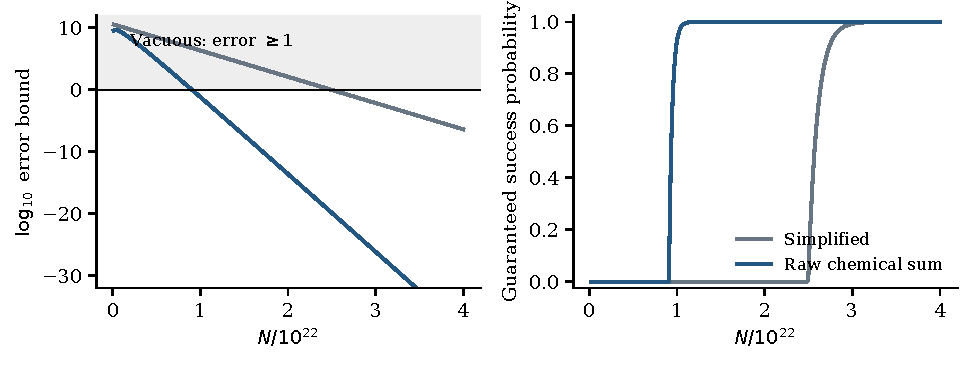
\includegraphics[width=\linewidth]{bounds.pdf}
\caption{Certified error formulas (left, logarithmic scale; the shaded band is vacuous) and the corresponding guaranteed success probability $\max(0,1-\tot)$ (right) for the parameters of Table~\ref{tab:example}. Both population tails are included; they are invisible at this scale.}
\label{fig:bounds}
\end{figure}

\paragraph{Margins.}
The selection margin $\frac35\log4-\log2-s=\frac15\log2-s$ is positive for $0<s<\frac15\log2\approx0.1386$; increasing the demanded gain consumes it linearly (Figure~\ref{fig:consequences}, middle). The deadline margin $\frac9{40}\gamma T-\log4$ is positive for $\gamma T>\frac{40}9\log4\approx6.161$. Beyond that, a longer horizon reduces the deadline tail exponentially but increases the chemical term linearly in $T$, so a longer batch is not automatically a stronger certificate (Figure~\ref{fig:consequences}, right).

\begin{figure}[ht]
\centering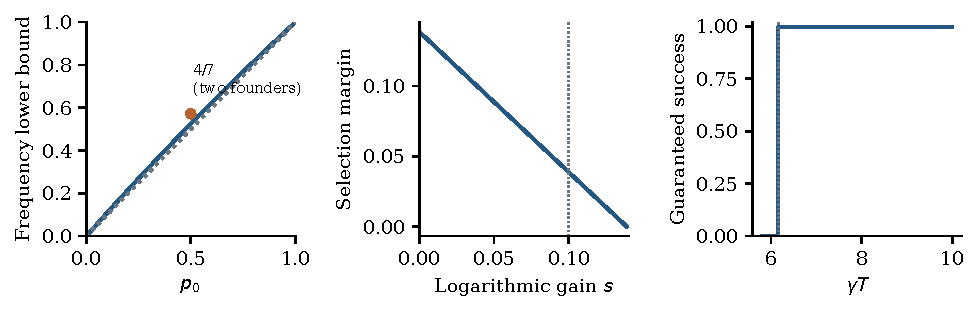
\includegraphics[width=\linewidth]{consequences.pdf}
\caption{Consequences of Theorem~\ref{thm:family}. Left: the $s=0.1$ frequency bound \eqref{eq:frequency} with the two-founder point $4/7$. Middle: the selection margin as a function of the demanded gain; its product with $\theta N$ is the negative logarithm of $\Esel$. Right: the guaranteed success probability against $\gamma T$ for $N=1.11\times10^{22}$, $M=2$, $\gamma=10^{-11}$, $s=0.1$; the dotted line marks the zero deadline margin. All curves evaluate proved expressions.}
\label{fig:consequences}
\end{figure}

\section{Discussion}\label{sec:discussion}

\paragraph{What the theorem establishes.}
For the specified effective model, a heritable difference in resident composition produces an advantage in compartment number, not merely in accumulated material, under a shared and depleting resource, with all descendants proved to remain in the state of their founder and with explicit error terms. The mechanism is entirely internal to the model: the high state holds about three times the $z$ concentration, grows about three times as fast per unit size, and this converts into at least a $\frac15\log2$ logarithmic gain in count odds after a factor two is paid for the phase mixture of an asynchronously dividing population. That factor is not an artefact of the proof; a small-exposure diagnostic in which both founders remain undivided shows that faster size growth need not change counts at all, so any bound on count odds must pay for phase.

\paragraph{What it does not establish.}
The scope is one batch and one nutrient hitting event. Endpoint compartments have arbitrary division phases and need not lie in the admitted newborn regions, so the gain cannot be compounded over serial transfers without a separate transfer-and-return theorem; fixation, spontaneous innovation, indefinite fidelity and autonomous membrane mechanics are outside the result. The size coordinate is proportional to volume by assumption. The resident feeds are maintained and only the growth precursor is finite. The reaction table is not atom-balanced and is not calibrated to any laboratory system; Table~\ref{tab:interpret} lists what would have to be identified before the model could be applied experimentally. The certified copy numbers are astronomically large because the certificates are conservative at every step (quadratic energy bounds, worst-case rates over the safe box, union bounds); nothing here suggests that the true failure probability behaves like the bound.

\begin{table}[ht]
\centering\small
\caption{Interpretation required before an experimental application.}
\label{tab:interpret}
\begin{tabular}{>{\raggedright\arraybackslash}p{.24\linewidth}>{\raggedright\arraybackslash}p{.68\linewidth}}
\toprule
Quantity & Interpretation or measurement\\
\midrule
$m,N$ & Calibrated coarse size coordinate proportional to volume; no membrane geometry is supplied.\\
$n_z/m$ & Growth-linked resident concentration in the chosen reference units.\\
$Q/\Omega$ & Well-mixed shared precursor concentration accessible to all compartments.\\
$\gamma$ & Growth coupling with its physical time and concentration units; the theorem needs $\gamma\leq10^{-11}$ in resident-rate units.\\
$10n_z-n_B$ & Chemical-state classifier; measurement error must be smaller than the sign margin at the endpoint.\\
Complementary partition & Independent allocation across species, fair allocation per molecule, conservation across the daughter pair.\\
Maintained exchanges & External feed and removal rates, and omitted reservoir driving, sufficient to sustain the propensities of Table~\ref{tab:rates}.\\
\bottomrule
\end{tabular}
\end{table}

\paragraph{Relation to Moran-type populations.}
The population of \citet{matsubara2026}, Appendix F, keeps its size constant by removing a random compartment at each division, as in the Moran process \citep{moran1958}, and reads selection from the resulting frequency dynamics. Here the population grows from $M$ to between $2M$ and $4M$ compartments, no compartment is removed, and the batch ends when the shared pool is depleted. The two settings ask different questions; the present one is closer to a serial-transfer protocol between transfers, and its output is a certified odds gain per batch rather than a fixation probability.

\paragraph{Open questions.}
(1) A transfer-and-return theorem: show that endpoint compartments, after a prescribed dilution and recovery step, re-enter the admitted newborn regions with explicit probability, so that the odds gain compounds over batches. (2) Sharper constants: the local recovery rate $k=u/672$ and the barrier $e^{16u}$ are far from tight; a certificate with $N$ of order $10^{8}$ rather than $10^{20}$ would change the practical meaning of the result. (3) More than two states, or states differing in species other than the growth-linked one. (4) Growth laws in which the precursor enters through a saturating or transport-limited rate rather than \eqref{eq:growth}. (5) A formalized trajectory-space construction that would move Section~\ref{sec:localization} into the machine-checked part.

\appendix

\section{Source certificate on the critical proof path}\label{app:cert}
In the coordinate order $(A,B,z,\Hs)$ the energy matrices are
\begin{align*}
P_L&=10^{-6}\begin{pmatrix}
1115801&-613708&2346047&3444885\\
-613708&1111499&-2339313&-3434384\\
2346047&-2339313&6767757&10178806\\
3444885&-3434384&10178806&15517433
\end{pmatrix},\\[4pt]
P_H&=10^{-6}\begin{pmatrix}
846084&-1159490&2352853&3510058\\
-1159490&4333988&-6781643&-10233028\\
2352853&-6781643&11398763&17222276\\
3510058&-10233028&17222276&26082111
\end{pmatrix}.
\end{align*}
Exact rational sum-of-squares decompositions give
\[
\tfrac1{200}\|y\|^2\leq y^{\!\top}P_Ly\leq24\|y\|^2,\qquad \tfrac1{200}\|y\|^2\leq y^{\!\top}P_Hy\leq42\|y\|^2 .
\]
For the root boxes \eqref{eq:roots} the symmetrized linearized drift contributes at most $-0.84\|y\|^2$ and the cubic remainder at most $0.25\|y\|^2$ when $|y_i|\leq1/400$, so $2y^{\!\top}P_if(x_i^*+y)\leq-0.59\|y\|^2$; the outer energy bound $E_i<b$ implies exactly this coordinate box, and the box in turn gives $n_k\leq70N$ and \eqref{eq:zsafe}.

\paragraph{Finite counts.}
A resident jump $\nu_r$ changes the energy by $2y^{\!\top}P_i\nu_r/m+\nu_r^{\!\top}P_i\nu_r/m^2$. The literal count propensities differ from their limiting values by the retained $1/m$ corrections. On the safe box the total resident propensity per unit size is at most $200000$, and the increments satisfy $(2y^{\!\top}P_i\nu_r)^2\leq100000\|y\|^2$ and $0\leq\nu_r^{\!\top}P_i\nu_r\leq210$. Applying $e^{v}-1\leq v+v^2$ for $|v|\leq1$ with $\alpha=10^{-12}$, summing the thirteen rate-weighted increments, and including the growth dilution jump gives
\begin{equation}\label{eq:preaffine}
\cL_{\mathrm{cell}}e^{\alpha NE_i}\leq\alpha e^{\alpha NE_i}\Big[-\frac N4\|y\|^2+200000000+8000000000N\beta^2\Big].
\end{equation}
The threshold $N\geq1.4\times10^{20}$ and $\beta\leq10^{-11}$ give $200000000+8000000000N\beta^2\leq Na/672$. If $E_i\geq a/2$, then $\|y\|^2\geq E_i/42$ bounds the bracket by $-Na/672$; if $E_i<a/2$, then $e^{\alpha NE_i}\leq e^{u/2}$. Adding $ke^{\alpha NE_i}$ to both sides in the second case yields \eqref{eq:local}.

\paragraph{Growth ratio.}
A growth event maps $y$ to $y'=y-(x+e_z)/(m+1)$. On the safe box $-2y^{\!\top}P_i(x+e_z)\leq36$ and $(x+e_z)^{\!\top}P_i(x+e_z)\leq211722$; with $N\leq m$ these give $\alpha N(E_i(y')-E_i(y))\leq\frac12$ and $e^{1/2}\leq2$, the factor two in \eqref{eq:local}, also for the growth event that triggers division.

\paragraph{Spatial and reset constants.}
$32\gamma\lambda\leq\alpha a/1344$ for $\gamma\leq10^{-11}$; $(4\alpha a-\lambda)N\leq-4479965/32$ at $N=1.4\times10^{20}$, which gives $2e^{4u-\lambda N}\leq1$; and $42\cdot16\delta^2<a$ for the partition perturbation.

\paragraph{Lattice rounding.}
For $N\geq10^{12}$, rounding $Nx_i^*$ coordinatewise to an integer count (with a small positive offset in the first coordinate) gives a newborn with $E_i(n/N)\leq4a$, so both newborn regions are nonempty far below the main threshold. Exact finite-count nonnegativity, the root signs, the rational energy decompositions and the inequalities above are the source certificates consumed by the population proof; no sampled trajectory or search history is part of the argument.

\section{Elementary inequalities}\label{app:ineq}
\begin{enumerate}[label=(\roman*)]
\item For $B\geq1000$: $\frac{999}{1000}\leq B\log(1+1/B)\leq1$. The upper bound is $\log(1+x)\leq x$; the lower bound is $\log(1+x)\geq2x/(x+2)$ for $x\geq0$, which at $x=1/B$ gives $2B/(2B+1)\geq\frac{999}{1000}$ for $B\geq1000$.
\item For $B_H,B_L\geq1000$, $W=B_H+B_L$, $a_H\in[2.97,3]$ and $a_L\in[0.99,1.01]$, item (i) gives $a_HB_H\log(1+1/B_H)-a_LB_L\log(1+1/B_L)\geq2.97\cdot\frac{999}{1000}-1.01=1.95703\geq\frac{39}{20}$, $(a_HB_H+a_LB_L)\log(1+1/W)\leq3W\cdot\frac1W=3$, and $(a_HB_H+a_LB_L)\log(1+1/W)\geq0.99\,W\log(1+1/W)\geq0.99\cdot\frac{999}{1000}\geq\frac{49}{50}$.
\item For $|v|\leq1$: $e^{v}-1\leq v+v^2$; and for the jumps of Lemma~\ref{lem:odds}, $|v_H|,|v_L|\leq\theta N(1/B_H+\frac35/W)\leq\frac{8}{5}\theta\leq\frac1{625}$ and $B|v|\leq\frac{8}{5}\theta N$, so $a_HB_Hv_H^2+a_LB_Lv_L^2\leq2\cdot3\cdot\frac{1}{625}\cdot\frac{8}{5}\theta N\leq\frac{6N}{390625}$.
\item For the deadline jump $v=-\theta N\log(1+1/W)$ with $W\geq NM\geq2N$: the linear part is at most $-\theta N\cdot\frac{49}{50}$ and the quadratic part at most $3W\theta^2N^2/W^2\leq\frac32\theta^2N$, so $(a_HB_H+a_LB_L)(e^{v}-1)\leq-\frac{9N}{10000}$.
\item Logarithmic margins: $0.69\leq\log2\leq0.70$, hence $\theta N[\frac15\log2-0.1]\geq\frac{19N}{500000}$ and $-\frac{9}{5000}N+\theta N\log4\leq-\frac N{2500}$.
\item Chemical envelopes: $\lambda=10^{-15}\geq\frac72\alpha a=\frac72\cdot\frac{10^{-12}}{5.12\times10^{8}}$ and $\delta^2/35=\frac{10^{-12}}{35}\geq\frac32\alpha a$; and $u\leq e^{u}$, $u\leq2e^{u/2}$ for $u\geq0$.
\end{enumerate}

\section{Formal statements and reproducibility}\label{app:formal}
The formal development is in Lean~4 \citep{demoura2021} with Mathlib \citep{mathlib2020}, toolchain version 4.30.0 (\texttt{leanprover/lean4}), with a frozen dependency manifest (SHA-256 \texttt{a8df0b60\ldots}). The verification bridge compiles the target and all local dependencies at their current source hashes, treats compiler warnings as errors, and records the axioms used by each exported declaration; every declaration listed below uses only \lean{propext}, \lean{Classical.choice} and \lean{Quot.sound}, with no \lean{sorry} and no additional axiom. All modules are under \lean{proofs/ResourceLimitedCompetition/} in the namespace \lean{ResourceLimitedCompetition}, and the finite-kernel and source-certificate infrastructure is imported from the earlier development in \lean{proofs/HeritableCompositions/} and \lean{proofs/FiniteCopy/}.

\paragraph{Endpoint statements.}
The theorem \lean{source_resource_limited_competition} in \lean{Main.lean} states: there exist $z_L,z_H$ in the intervals \eqref{eq:roots} that are stationary for the source rates; for every $M$ and $\gamma$ the error \lean{competitionError} tends to zero as $N\to\infty$; and for every $0<\gamma\leq10^{-11}$, every $N\geq1.4\times10^{20}$ and every $h,\ell\geq1$, the newborn regions are nonempty and, for every founder population in them, there is a clock $q$ dominating all rates such that the Poissonized stopped kernel at time $q\cdot8/\gamma$ assigns the success set \lean{competitionSuccessSet} probability at least one minus \lean{competitionError}, the right-hand side of \eqref{eq:original}. The success set is exactly the event $\cS_{0.1,8/\gamma}$ of Section~\ref{sec:stopped} as a set of terminal records. The theorem \lean{source_resource_limited_tradeoff} in \lean{SourceTradeoff.lean} is the same statement with an arbitrary real gain and an arbitrary nonnegative horizon $t$ and the error $\chem(N,M,t)+\Esel(N,s)+\Etime(N,\gamma,t)$, that is, Theorem~\ref{thm:family}. Both are obtained from the population theorems \lean{finite_batch_competition} and \lean{finite_batch_tradeoff}, which take an arbitrary admitted founder population as hypothesis. Table~\ref{tab:formal} maps the steps of this paper to modules and principal declarations.

\begin{table}[p]\centering\footnotesize
\caption{Critical-path formal source map (namespace \texttt{ResourceLimitedCompetition}).}\label{tab:formal}
\begin{tabular}{>{\raggedright\arraybackslash}p{0.34\textwidth}>{\raggedright\arraybackslash}p{0.58\textwidth}}\toprule
Step in this paper & Modules and principal declarations\\\midrule
Population states, conservation (Lemma~\ref{lem:conservation}) & MembraneConservation: \lean{step_conservation}, \lean{resource_population_budget}, \lean{resource_endpoint}\\
Finite active domain, stopped kernel (Section~\ref{sec:finitelaw}) & FinitePopulation, StoppedPopulation, PopulationSupport, NutrientEndpoint: \lean{activeDomain}, \lean{stoppedPopulationModel}, \lean{positive_active_domain_preserved}\\
Comparison lemmas (Lemmas~\ref{lem:barrier}, \ref{lem:union}) & DeadlineProbability, ProbabilityUnion, UnflaggedProbability: \lean{poissonized_barrier}, \lean{poissonized_event_cover}, \lean{probability_complement_lower}\\
Local estimate \eqref{eq:local} & AffineGrowthGenerator, SourceDivisionBarrier: \lean{low_resource_local_affine}, \lean{high_resource_local_affine}, \lean{low_source_growth_ratio}\\
Position exponential (Lemma~\ref{lem:spatial}) & DivisionBarrier, SourceSpatial, SpatialReset, CellSpatial: \lean{compartment_spatial_bound}, \lean{spatial_pair_reset}\\
Division-energy failures (Lemma~\ref{lem:division}) & SpatialPopulationBoundary, GlobalSpatial: \lean{global_division_failure_bound}\\
Outer failures (Lemma~\ref{lem:outer}) & CellOuter, OuterPopulationBoundary, GlobalOuter, OuterFailure: \lean{global_outer_failure_bound}\\
Partition failures (Lemma~\ref{lem:partition}) & CellPartition, PartitionEvent, PartitionPopulation, GlobalPartition: \lean{cell_partition_failure}, \lean{global_partition_failure_bound}\\
Chemical error (Proposition~\ref{prop:chem}) & ChemicalBranchCombination, ChemicalTailScalar, ChemicalProbability: \lean{global_chemical_probability}, \lean{chemical_raw_envelope}\\
Ancestral totals, odds observable (Lemma~\ref{lem:odds}) & AncestralMembrane, AncestralRates, PopulationLogBounds, PopulationOddsDrift, GlobalOdds, OddsProbability, GainProbability: \lean{global_odds_generator}, \lean{global_gain_probability}\\
Size odds to count odds (Lemma~\ref{lem:endpoint}) & EndpointOdds, GainEndpoint, NutrientOdds, GainNutrient: \lean{count_to_membrane_odds}, \lean{endpoint_gain_barrier}\\
Deadline (Lemma~\ref{lem:deadline}) & DeadlineScalar, DeadlineValue, GlobalDeadline, DeadlineProbability, DeadlineFamily: \lean{global_deadline_probability}, \lean{deadline_probability_family}\\
Coverage and assembly (Section~\ref{sec:assembly}) & SuccessCoverage, EnrichmentCoverage, FiniteBatchCompetition, Tradeoff: \lean{competition_failure_coverage}, \lean{finite_batch_competition}, \lean{finite_batch_tradeoff}\\
Source instantiation, error decay & Founders, ErrorDecay, Main, SourceTradeoff: \lean{source_births_nonempty}, \lean{competition_error_tendsto_zero}, \lean{competition_error_threshold}, \lean{source_resource_limited_competition}, \lean{source_resource_limited_tradeoff}\\
Corollary~\ref{cor:frequency} & Frequency: \lean{odds_implies_frequency}, \lean{frequency_gain_identity}, \lean{success_two_founder_frequency}\\
Corollary~\ref{cor:sharp} & SharperError: \lean{chemical_raw_sharp}, \lean{chemical_raw_double_exponent}\\
Proposition~\ref{prop:thresholds} & AccuracyScaling: \lean{chemical_joint_envelope}, \lean{three_tail_accuracy}, \lean{joint_scaling_decay}\\
Weight identities of Section~\ref{sec:localization} & JointLocalization: \lean{growth_sizeWeight}, \lean{complementary_sizeWeight}, \lean{joint_weight_drift}\\
\bottomrule
\end{tabular}
\end{table}

\paragraph{Receipts.}
The strict verification of \lean{Main.lean} (declarations \lean{source_resource_limited_competition}, \lean{finite_batch_competition}, \lean{competition_error_threshold}) compiled with empty compiler output in $97.5$~s with $108$ authenticated local dependencies; the aggregator \lean{PostProof.lean}, which imports the modules of Table~\ref{tab:formal} added after the main theorem, compiled with empty output in $126.4$~s with $120$ authenticated dependencies, and a replay of the unchanged \lean{Main.lean} in the same session took $30.6$~s. Source SHA-256 of \lean{Main.lean}:
\begin{center}\footnotesize\ttfamily
72b01179fc4a7b8667be927eed6ef8b89a609eddc9a02386b11a0b7ddf20a9e1
\end{center}
and of \lean{PostProof.lean}:
\begin{center}\footnotesize\ttfamily
9a8ff23b3b1fb067e18952e158ab6b372a6c7ecf7d066285b3d8d23d7c31c5a3 .
\end{center}
Within the development, verification is reproduced from the repository root by
\begin{quote}\footnotesize\ttfamily
python scripts/verify\_proof.py proofs/ResourceLimitedCompetition/PostProof.lean \textbackslash\\
\hspace*{2em}--timeout 600 --output RECEIPT.json
\end{quote}
which pins the working directory and toolchain. Hashes document correspondence between the receipts and the sources; they are not mathematical evidence by themselves.

\paragraph{Formal scope.}
Lean verifies: the finite stopped law and its Poissonized kernel; the conservation identities; the source-local estimates \eqref{eq:local} for both compositions on the literal count generator including the $1/m$ corrections; the position exponential and the daughter reset; the three chemical failure bounds and their sum; the ancestral-total observables, their generator inequalities and endpoint conversions; the deadline bound; the coverage of the failure set; the union bound; the source instantiation with nonempty newborn regions; Theorems~\ref{thm:family} and \ref{thm:main}; Corollaries~\ref{cor:frequency} and \ref{cor:sharp}; Proposition~\ref{prop:thresholds}; and the weight-preservation and linear-drift identities used in Section~\ref{sec:localization}. Conventional: the nonexplosion and coupling argument of Section~\ref{sec:localization}, the small-exposure diagnostic mentioned in Section~\ref{sec:discussion}, and the interpretations of Table~\ref{tab:interpret}. The decimal entries of Table~\ref{tab:example} and the figures are directed-interval or floating-point evaluations of proved formulas and are not kernel evidence.

\bibliographystyle{plainnat}
\bibliography{refs}

\end{document}
